\documentclass[UKenglish]{beamer}


\usetheme[NoLogo]{MathDept}


\usepackage[utf8]{inputenx} % For æ, ø, å
\usepackage[spanish]{babel}          % Automatic translations
\usepackage{csquotes}       % Quotation marks
\usepackage{microtype}      % Improved typography
\usepackage{amssymb}        % Mathematical symbols
\usepackage{mathtools}      % Mathematical symbols
\usepackage{graphicx}
\usepackage[absolute, overlay]{textpos} % Arbitrary placement
\setlength{\TPHorizModule}{\paperwidth} % Textpos units
\setlength{\TPVertModule}{\paperheight} % Textpos units
\usepackage{tikz}
\usetikzlibrary{overlay-beamer-styles}  % Overlay effects for TikZ


\author{Rudik Roberto Rompich}
\title{Wilkinson Microwave\\ Anisotropy Probe}
\subtitle{\texttt{Introducción a la astronomía}}


\begin{document}

{\usebackgroundtemplate{%
  \includegraphics[width=\paperwidth,height=\paperheight]{wmap.png}}
\section{WMAP}
\SectionPage 
\usebackgroundtemplate{ } 

\section{Índice}


% Use
%
%     \begin{frame}[allowframebreaks]{Title}
%
% if the TOC does not fit one frame.
\begin{frame}{Índice}
    \tableofcontents[currentsection]
\end{frame}


\section{Sonda}

\begin{frame}
\frametitle{Sonda}{\textbf{Punto de Lagrange}}

\begin{columns}

\column{0.4\textwidth}
La sonda se ubica en el punto:
$$\mathcal{L}=2$$
Es decir: 

\begin{itemize}
\item A 1.5 millones km de la tierra.
\item Lado opuesto del sol.
\end{itemize}

\column{0.4\textwidth}

  \begin{figure}[h!]
    \centering
    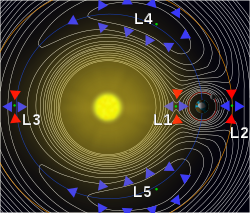
\includegraphics[scale=0.5]{lagrange.png}
    \caption{Puntos de Lagrange}
    \label{fig:punt4os}
    \end{figure}
\end{columns}
\end{frame}


\begin{frame}
\frametitle{Sonda}{\textbf{Punto de Lagrange}}
\begin{figure}[h!]
    \centering
    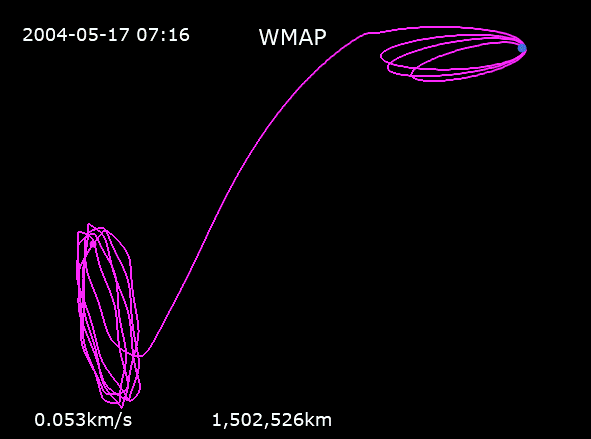
\includegraphics[scale=0.4]{real.png}
    \caption{Puntos de Lagrange}
    \label{fig:pun2tos}
    \end{figure}
\end{frame}
\begin{frame}
\frametitle{Sonda}{\textbf{Punto de Lagrange}}
\begin{figure}[h!]
    \centering
    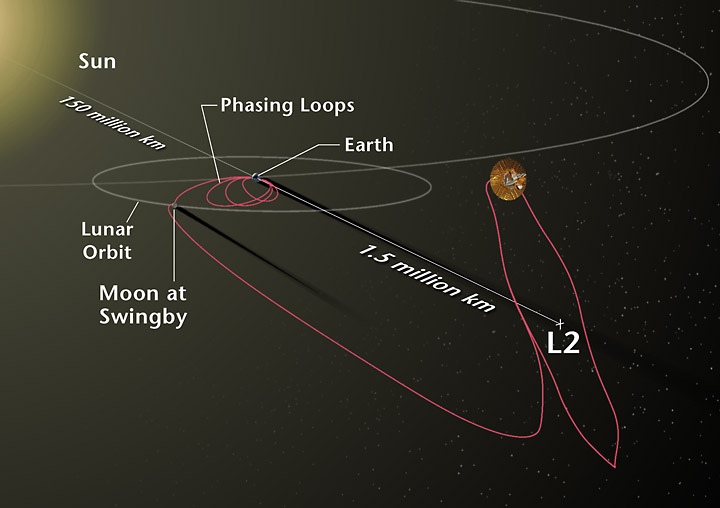
\includegraphics[scale=0.3]{trac.jpg}
    \caption{WMAP en $\mathcal{L}=2$}
    \label{fig:pu3ntos}
    \end{figure}
\end{frame}

\begin{frame}
\frametitle{Sonda}{\textbf{Descripción}}

\begin{columns}

\column{0.4\textwidth}
MAP. (2003) En honor a David Todd Wilkinson. \\
Puntos interesantes:
\begin{itemize}
\item NASA/Princeton.
\item 2001 a 2010 (Plank de ESA).
\item Temperatura del CMB. 
\item Anisotropia = facultades de la materia.
\end{itemize}

\column{0.4\textwidth}

  \begin{figure}[h!]
    \centering
    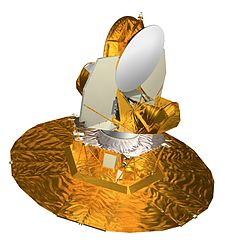
\includegraphics[scale=2]{sonda.jpg}
    \caption{Sonda}
    \label{fig:punto2s}
    \end{figure}
\end{columns}

\end{frame}
\begin{frame}
\frametitle{Sonda}{\textbf{Descripción}}

\begin{columns}

\column{0.4\textwidth}
\begin{figure}[h!]
    \centering
    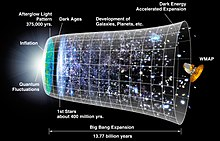
\includegraphics[scale=0.5]{sonda2.jpg}
    \caption{Sonda}
    \label{fig:puntos}
    \end{figure}

\column{0.4\textwidth}
    Principales objetivos
    \begin{itemize}
        \item Evolución
        \item Big Bang. 
        \item Teoría de la inflación.
    \end{itemize}
Descubrimientos: 
    \begin{itemize}
        \item Datos inusuales al modelo estándar de cosmología. 
    \end{itemize}
    \end{columns}

\end{frame}

\begin{frame}
\frametitle{Sonda}{\textbf{Imágenes}}
\begin{columns}[t]
\column{.5\textwidth}
\centering
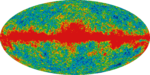
\includegraphics[width=4cm,height=3cm]{1.png}\\
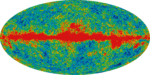
\includegraphics[width=4cm,height=3cm]{2.png}
\column{.5\textwidth}
\centering
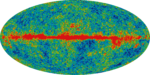
\includegraphics[width=4cm,height=3cm]{3.png}\\
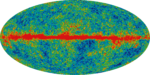
\includegraphics[width=4cm,height=3cm]{4.png}
\end{columns}
 
\end{frame}


\begin{frame}
\frametitle{Sonda}{\textbf{Evolución}}
\begin{figure}[h!]
    \centering
    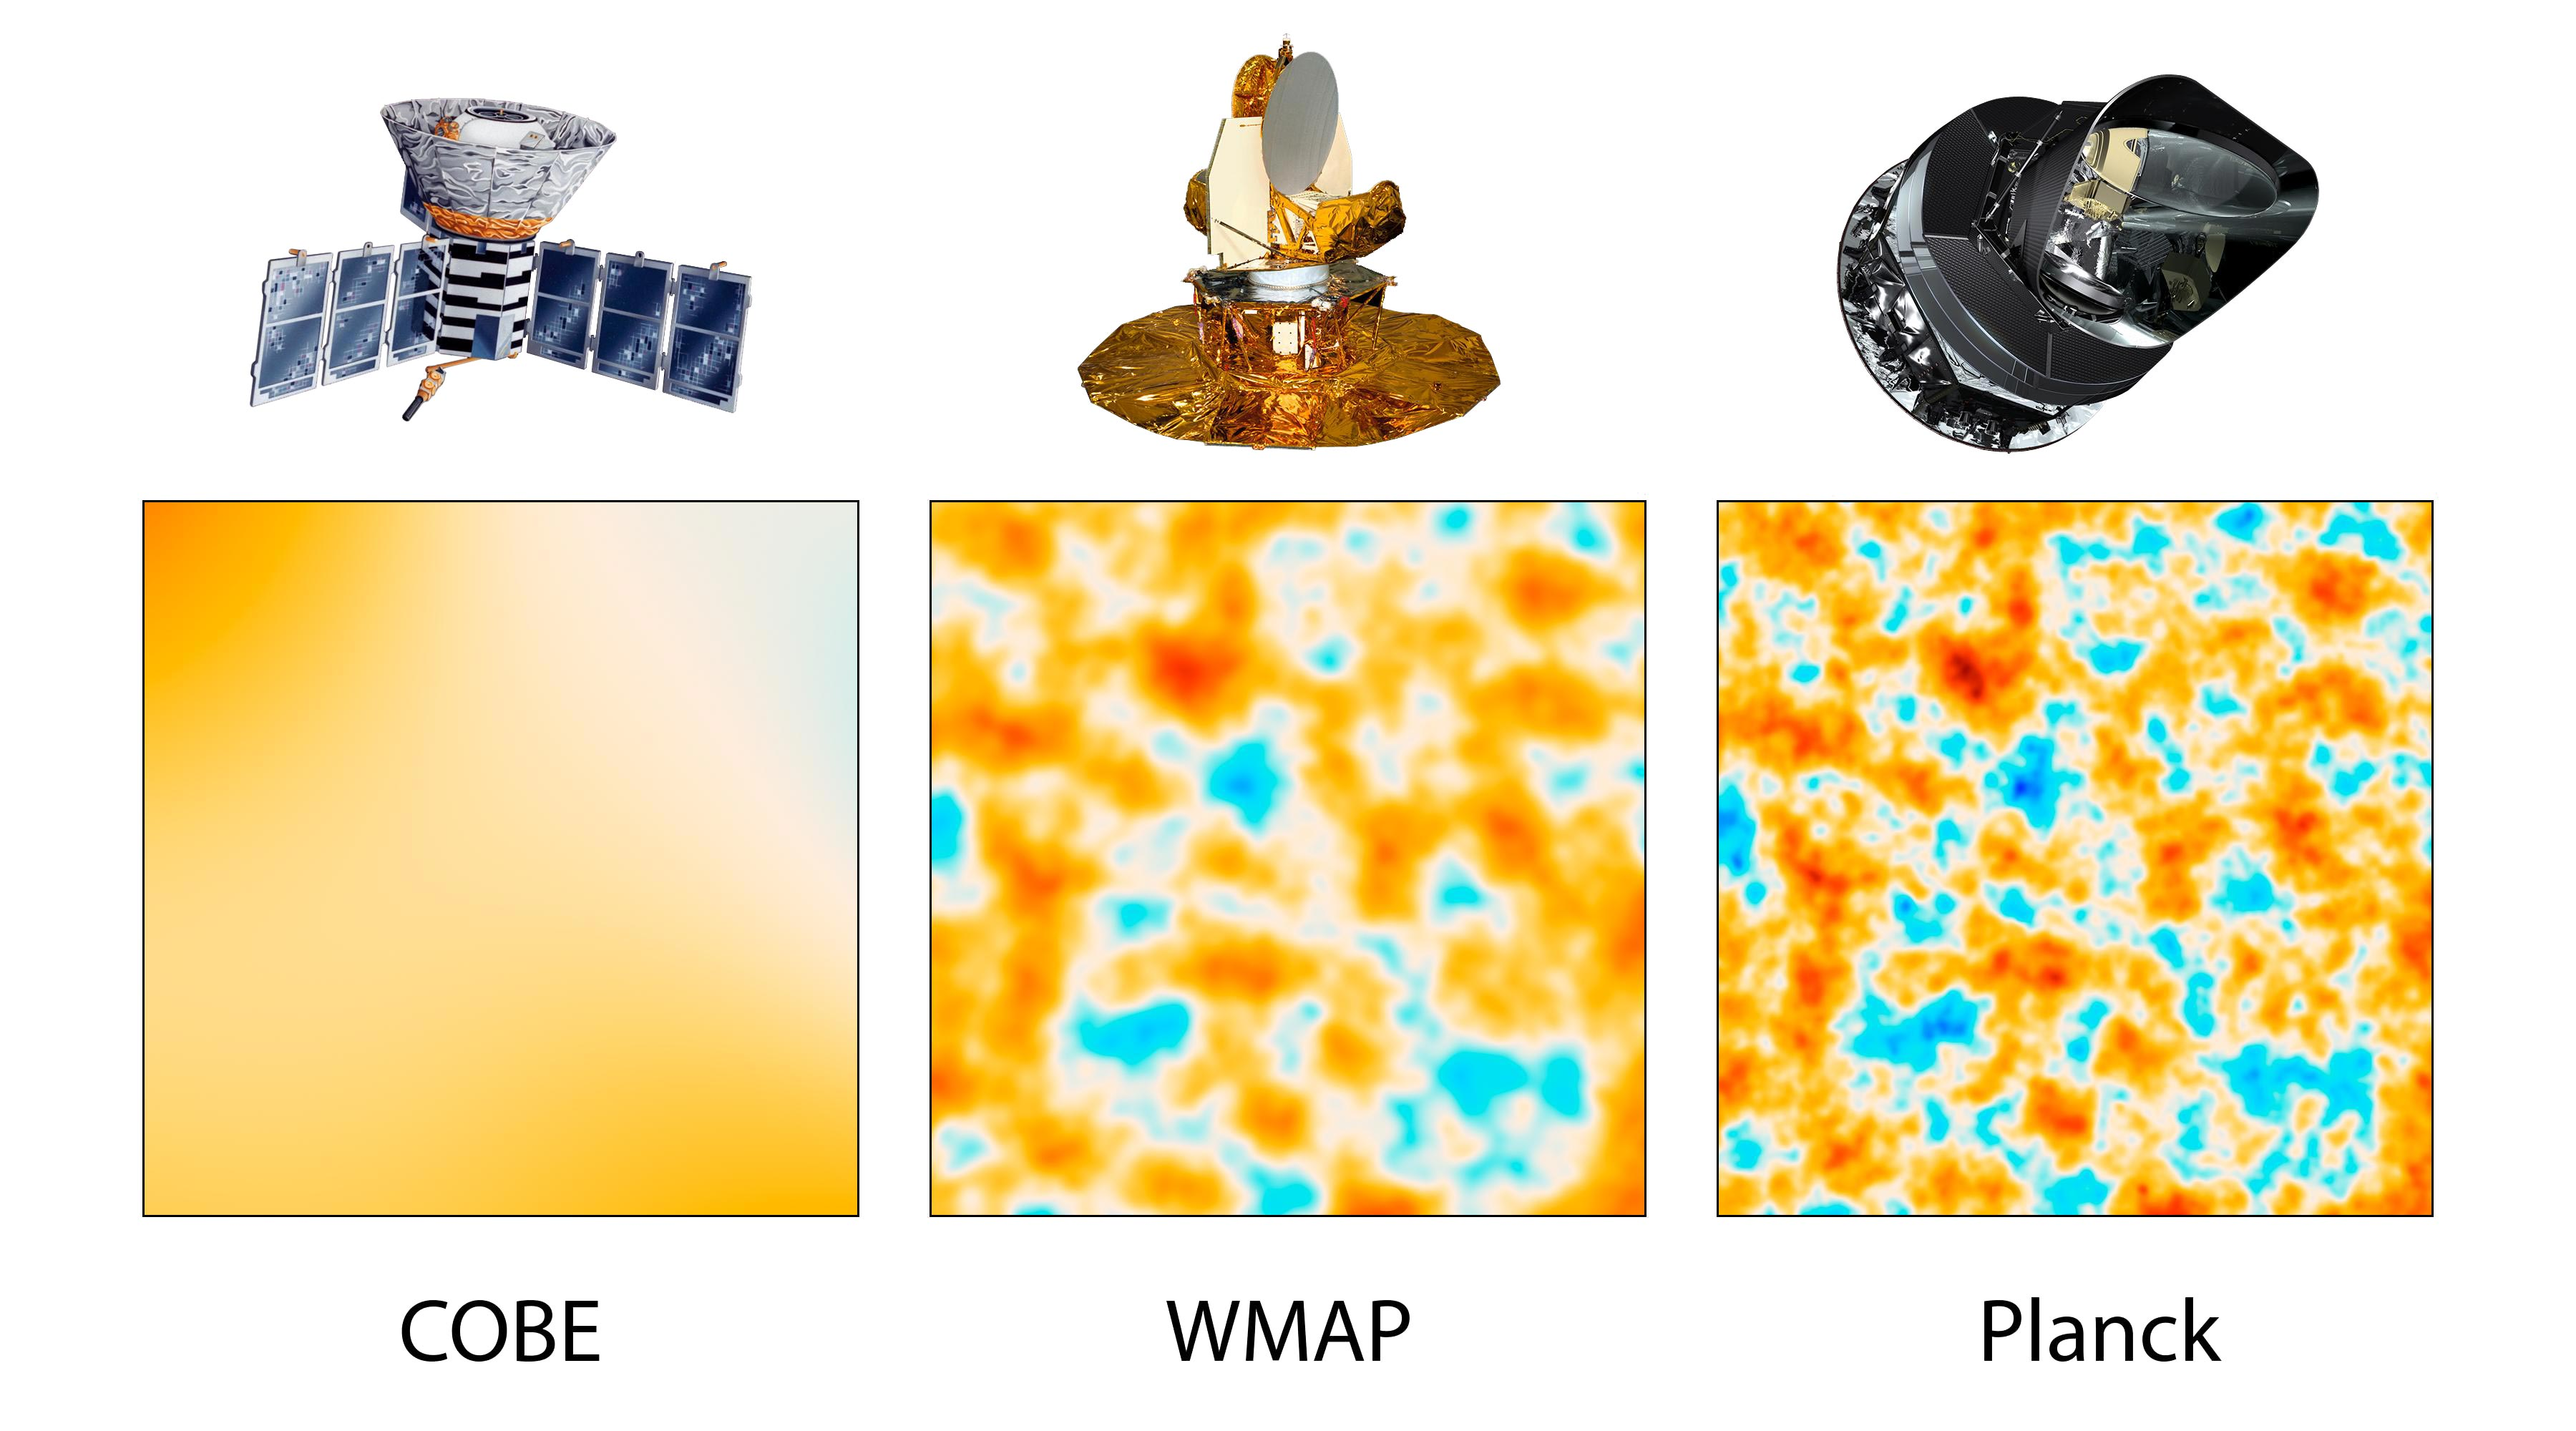
\includegraphics[scale=0.09]{lol.jpg}
    \caption{Evolución}
    \label{fig:jeje}
    \end{figure}
\end{frame}


\section{Referencias}
\begin{frame}[allowframebreaks]{Referecias}
    \begin{thebibliography}{}

        
        \bibitem{Helso2020}
        Goddard Space Flight Center.
        \newblock \enquote{Wilkinson Microwave Anisotropy Probe: Overview}.
        \newblock  04-08-2009.
        Recuperado de: https://lambda.gsfc.nasa.gov/product/map/current/
    

    \end{thebibliography}
\end{frame}


\end{document}